% --------------------------------------------------------------
% Abhi's Standard Preamble.
% --------------------------------------------------------------
 
\documentclass[12pt]{article}
 
%Packages
\usepackage[margin=1in]{geometry} 
\usepackage{graphicx}
\usepackage{url}
\usepackage{hyperref}
\usepackage{float}
\usepackage{quoting}

\usepackage{aurical}
 
\begin{document}
 
\title{Cort Ireheart, Arcane Shaper}
\date{}

\maketitle

%\Fontauri

\begin{figure}[H]
  \centering
  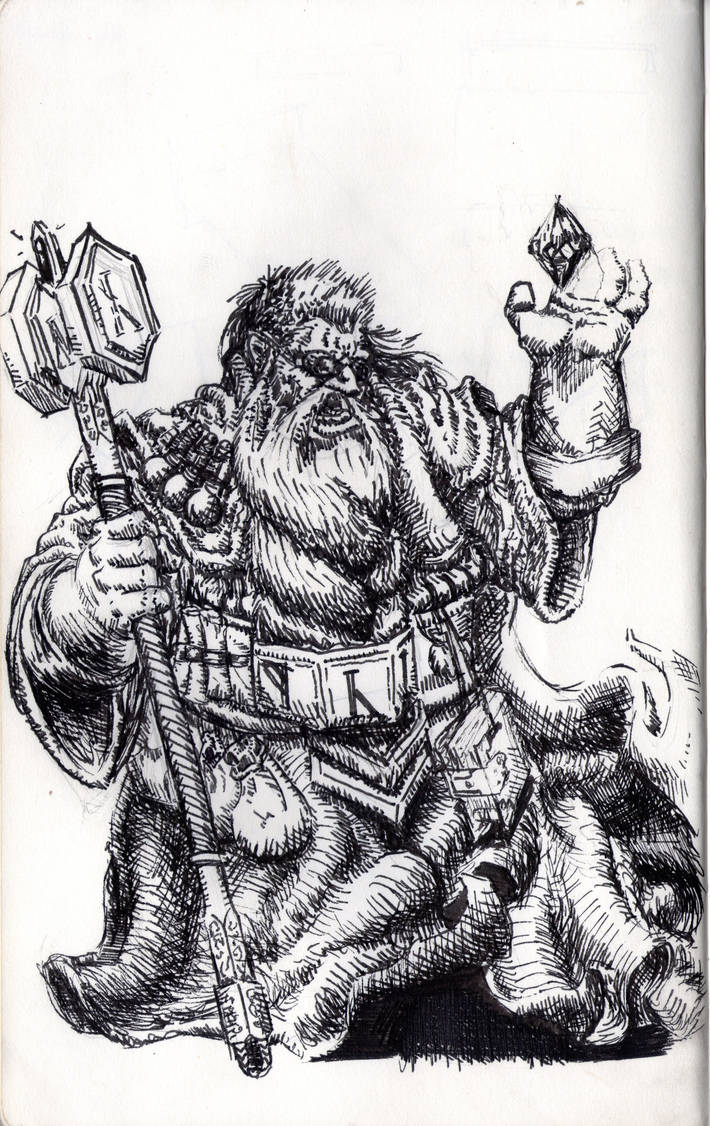
\includegraphics[width=.62\textwidth]{./resources/Cort_Ireheart.jpg}
  \caption{Cort's current appearance.}
\end{figure}

\section{Character Description}

Donning scale mail and a war-hammer almost his own size, many are surprised to
see the red robes underneath Cort's armor. Even more so when they realize he's
a dwarf. However, never having been one for tradition, Cort walks among the
surfacers as probably the only non black robed dwarven wizard. A craftsman
seeking the pinnacle of his art, he uses his transmutation based magic to
bolster his art in smithing and refining. When asked, he would say that he
adventures to find extrodinary materials to improve his hammer, and to give his
name resounding fame, to spite his bretheren from Thorbardin.

Cort stands 4 foot, 8 inches tall and is of stocky build, despite his prodigious
357 years of age. As mentioned before, he wears scale mail and wields a large
hammer, with many runes engraved upon it. The runes of the hammer seem to light
up when he's casting magic. He wears his red robes underneath his armor, though
the crest of the order of the Red Robes is branded onto the armor itself. He
also wears thick leather gloves on either hand, which conceals burned and
scarred hands, with fingers that seem to have been broken before. Strapped to
his belt is a deep red tome, with a crest depicting a tree bathed in red
moonlight. He never parts with the tome.

\begin{figure}[H]
    \centering
    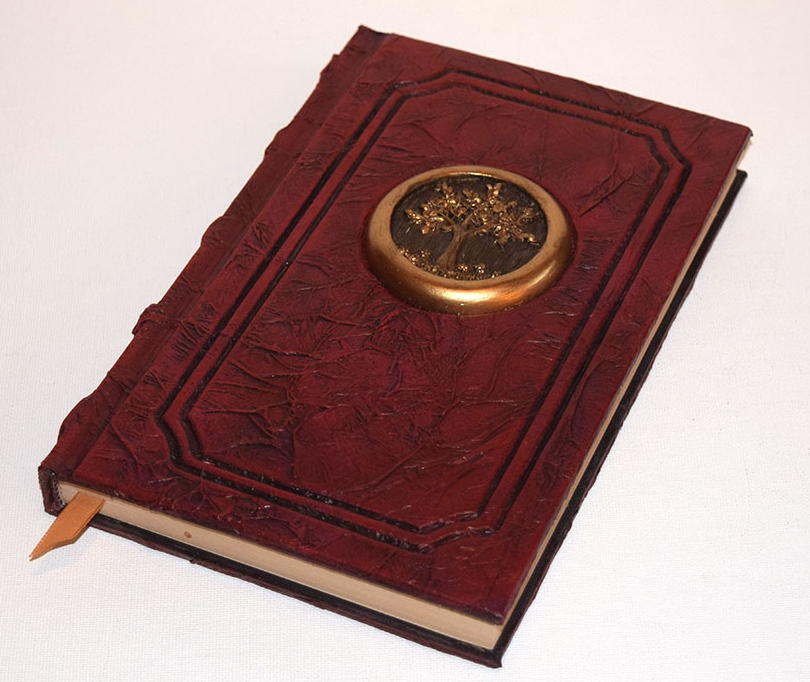
\includegraphics[width=.65\textwidth]{./resources/tome.jpg}
    \caption{The tome that Cort carries on his waist.} \label{fig:tome}
\end{figure}

In general, strangers will find Cort polite and friendly, but far from trusting.
It's hard for him to trust new people, so he will likely be wary in both manner
and action. However, to those who he trusts he is loyal to his death, which he
is not afraid of given his long life. Cort follows the philosophy of returning
good with good, and evil with evil and therefore is capable of acts falling into
both sides of the morality alignment. However, Cort will not start something on
his own without direct instigation, and treats people as kindly as possible. 

He has a strong hatred against overbearing families who treat their descendents
like political tools and holds an arrogant disdain against those who cling to
tradition, potentially to his detriment. In addition, he has a strong dislike
for those who hate or surpress magic without reason. However, he's very fond of
fellow craftsmen, mages regardless of robe, and of children (which is mostly
everyone relative to his own age). He won't give up an opporunity to learn, and
likes to spend time getting to know the local practitioners to deepen his skill.

\section{Backstory}

\subsection{Beginnings}

Born to the Ireheart clan, a major noble family among the Hylar Dwarves, Cort
was among the promising youth of the clan. The Ireheart's, as one might guess by
their namesake, was a clan of great warriors, whose great deeds of heroism and
strength resounded in Thorbardin centuries ago during the many wars the Dwarven
empire endured. The hope was that Cort too would grow to be a great warrior, and
he was trained as such, but due to a chance encounter with a Daewar grandmaster
craftsman who saw potential within the inquisitive Cort, Cort instead trained to
become a weapon and armor smith in the small school of learning that his master
established. This displeased his clan heavily, especially his parents, but
given that it was atleast a Daewar craftsman of great repute, they let it be.

During this initial century of his life, Cort toiled tirelessly, advancing from
an apprentice, to an initiate, to finally a craftsman of his own right. His
reputation grew as well, people knew him for his weapons and armor designed with
beautifully intricate engravings. This was perhaps the highest point of his
life, a time where his family accepted and reveled in his reputation, his works
were desired among many, chiefly his own clan, and he had time to improve
himself ceaselessly. However, it all came crumbling with a single text.

\subsection{The Red Tome}

A duty of the crafting guild Cort was a part of was to occasionally accompany
mining expeditions, to indentify and inspect veins of ore. One day, Cort was out
on such a expedition, when disaster struck. The entire cavern began to shake,
the walls, ceilings, and even ground began to collapse as the party slowly began
to be buried by stone. Furiously, the group rushed towards safety, but Cort
was unluckily struck by a falling rock and sunk into unconsciousness as he was
buried by stone.

\begin{figure}[!htb]
    \centering
    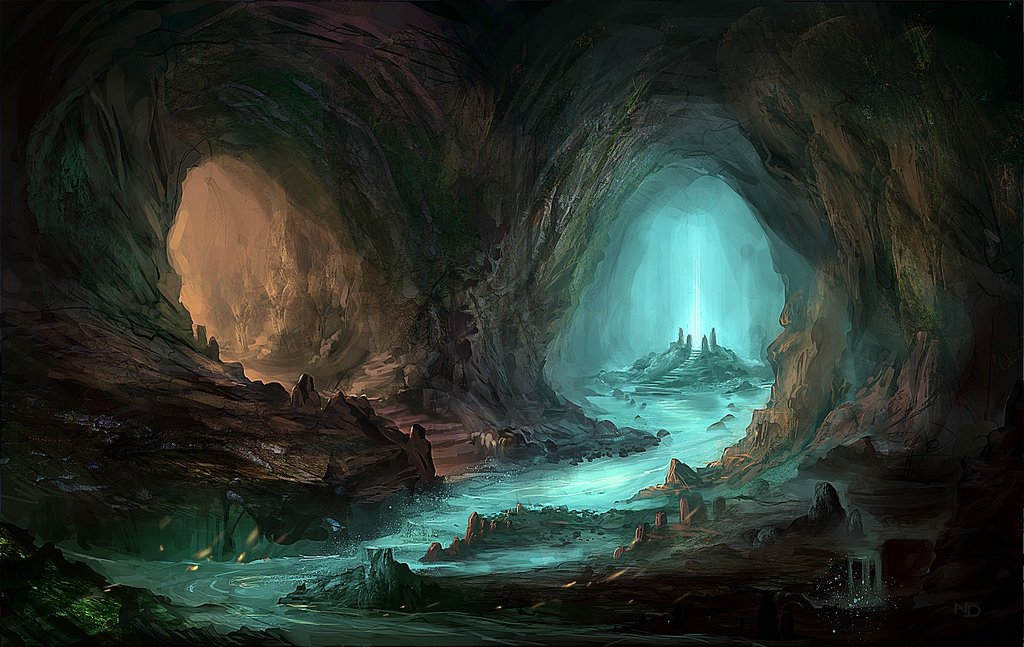
\includegraphics[width=\textwidth]{./resources/cavern}
    \caption{The cavern Cort awoke in.} \label{fig:cavern}
\end{figure}

When he awoke, some unknown amount of time later, he found himself in a small
cavern (see figure \ref{fig:cavern}), no sign of the previous tunner he was in.
At the end of this cavern was a small river, which was fed by a small waterfall,
underneath which was some kind of stone stele. Cort, inquisitive by nature,
ignored his injuries to investigate the stele, and upon arriving to it, noticed
a small red tome floating atop it, half open (see figure \ref{fig:tome}). Upon
it, and also around the stele, was emblazoned a tree bathed in red moonlight.

Cort initially avoided the relic, as most dwarves hold great mistrust in the
matters of magic, not to mention his clan being extremely xenophobic to it. But
as minutes turned to hours, turned to days, Cort could not find an escape from
this seemingly enclosed cavern. His injuries worsened, his mental condition
worsened from the famine and despair. In the end, he could no longer avoid the
tome. Cautiously approaching it, he tried to peer at its contents, but could not
decipher the language. With no other option, Cort moved to hold the tome in his
hands, and in the moment was frozen in place as from nowhere, magical energies
rose from the stele and restrained him. The tome floated higher in front of him,
bathing him with red light, and from cover to cover flipped through the
contents. With each page turned, Cort felt his head pound and his body throb as
his constitution changed. He began to be able to \textit{feel} the magic
surrounding him, his natural resistance to magic fading and replacing it
a sensitivity normally only found in the Theiwar. 

Through the pain, Cort managed to lift his head and saw in the place of the book
stood a veiled maiden, clad in red robes. She smiled, and as distrusting as Cort
was, he only saw her kindness, perhaps with a hint of mischief. He heard her
speak, but to this day is hazy on the exact words spoken as he soon fainted.

He woke, later, in a bed in a Gully Dwarf slum. The two owners of the
establishment explained how they were miners who, during an expedition, saw him
literally fall through the ceiling, unconscious and grievously injured. Their
supervisors naturally didn't believe the bewildering words of the two Gully
Dwarves, but they nonetheless brought him back to be healed. Grateful for their
assistance and finding their company pleasant, ignoring their prodigious idiocy,
he became good friends with the two. However, when he was by himself, he noticed
that in his pack, the red tome had mysteriously appeared, this time, however,
with completely blank pages. However, his sensitivity to magic remained, and he
could feel that this was no ordinary item.

\subsection{Arcane Shaper}

After he had recovered, Cort traveled back to Thorbardin, along with his two new
friends, and enjoyed a joyous return to his family before immediately shutting
himself in seclusion. Fourty years he spent without a peep to society, who had
assumed he had become a recluse due to his accident. During this time he
explored and experimented on his heightened magic sensitivity, and discovered
that he had gained the ability to temporarily transmute materials into different
ones, not unlike the minor alchemy that wizards were spoke of to possess.

At first he was distraught, thinking himself a monster, but soon, an idea formed
in his invention-obsessed brain. Dashing across his workshop, he dug through
piles of materials until he found a few iron ingots. Melting them down into
a rod shape, he focused all of his powers to will them into a pliable wood,
which he reshaped into a recurve bow, clamping it in place. Then, releasing his
ability, he watched in amazement as the weak wooden bow slowly reformed itself
into iron. He picked up the bow, not daring to believe the sight. His eyes shown
with wonder and excitement.

\begin{figure}[!htb]
  \centering
  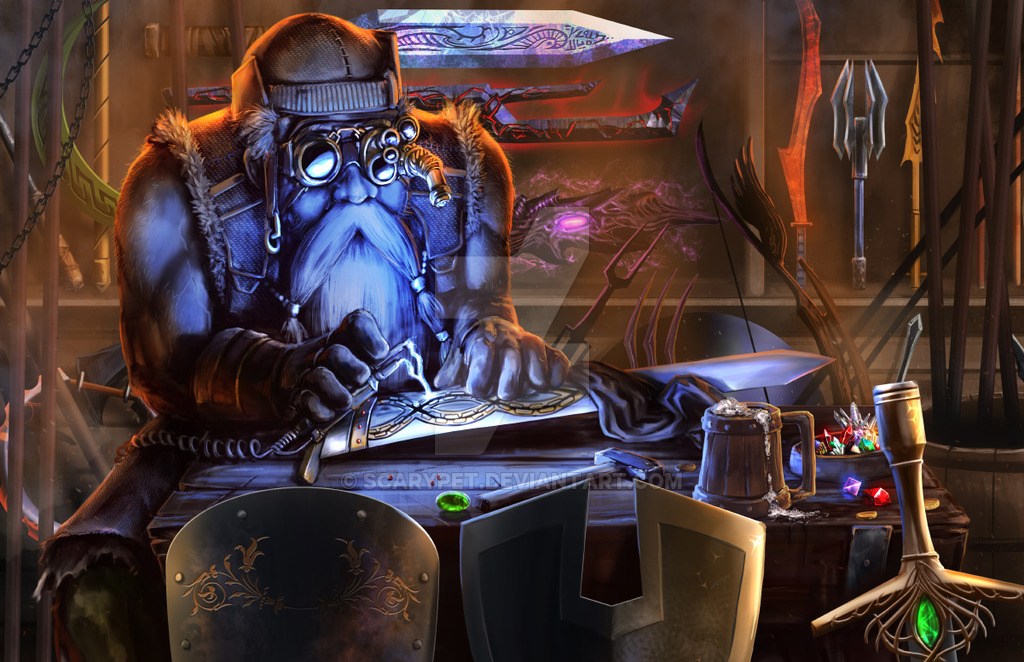
\includegraphics[width=\textwidth]{./resources/arcaneshaper}
  \caption{Cort working on his crafts, leveraging his new magic.}
\end{figure}

Cort spent these fourty years meticulously learning how to control his
transmutation ability, and apply it to his art. Turning metal into wood for easy
shaping was only one such feat, he could turn wood into metal to gain it's
malleability, turn heat resistant ones into ones less so to melt, create
fantastical alloys and blends. These wonderous combinations and experiments were
usually left on a wall in his workshop, but due to his mischevious gully dwarven
friends, a few made it out to the dwarven city, and started an uproar. 

Thorbardin, a city mistrustful of magic but still comprised of master craftsmen,
were stunned by these fantastical creations that leaked out. Incredible feats of
art, no one smith dared say that they could reproduce them, but of course they
didn't know that they were magically created. Each and every one of them were
branded with the same crest as Cort's text, but this created confusion in the
city as such a crest had never been publicly claimed.

Cort was perfectly content to spend the rest of his life researching his
creations, after all with his abilities he could spend his entire lifespan
creating and not exhaust the possibilities. However, soon a piece of news shook
Thorbardin, his master had died.

\subsection{The Grandmaster Selection}

When Cort learned his master had perished, he was naturally distraught. This was
the man that had taught him his craft. Showed him the pride of an artist. More
of a father to him than his biological dad. But imporantly, this boded ill for
all his master's apprentices. Without the grandmaster supporting them, they were
bound to lose funding from Thorbardin to continue having their work funded. This
set everyone, especially Cort into a panic. He had been consuming semi-rare
materials for his research for a long time now, and without the grant, he would
be stuck. Unable to progress. That was unacceptable. If the school couldn't
produce a new grandmaster, he himself had to step up.

\begin{figure}[H]
  \centering
  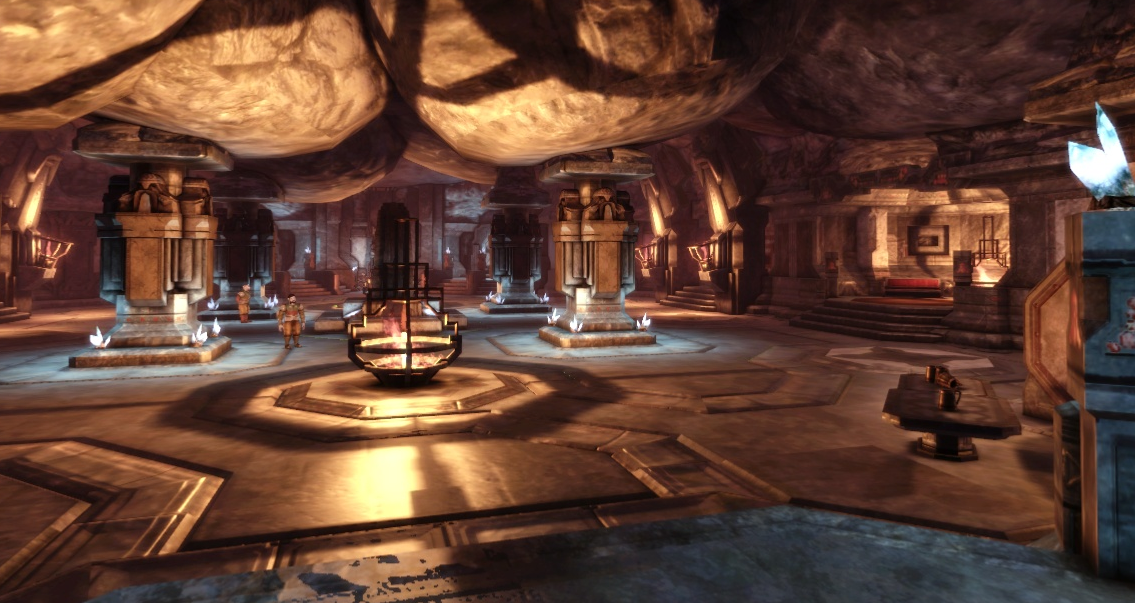
\includegraphics[width=\textwidth]{./resources/arena}
  \caption{The grandmaster exam arena.}
\end{figure}

But as he emerged from his seclusion to deal with the matter, he also heard the
rumors about the new fantastical materials and crafts going around, his crafts.
His pride swelled, and although he knew that using magic would be heavily
frowned upon, his ego prevented him from seeing this danger. He immediately
signed himself up to take the grandmaster's exam, a test which would be
conducted publicly in the arena for all to spectate.

Becase he had been in seclusion for so long, not many were drawn to his
examination, as many attempted to become a grandmaster and failed often as well.
However, his beloved Ireheart family and his friends from the academy did
attended. Standing alone in the middle of the arena, his task was to create
a hammer of the finest quality he could muster.

Cort, as usual tuned out his surroundings, and brought out his materials, ingots
of iron and silver as well as wooden pieces from a special tree with violet
colored bark, much to the bewilderment of the crowd. He began with the crown of
the hammer, made in the usual manner, at the moment displaying nothing special.
But then he began to weave his magic, shocking the crowd into silence,
transmuting the crown into wood, and using fine woodworkers tools to craft
intricate patterns, designs, and deadly spikes onto it. Furthermore, he took the
violet bark, turned it into common iron, and melted it down into a spiral mold,
somehow managing to create this hefty violet skinned coiled handle, which fit
directly into the crown. The result, although alien from the usual dwarven
creations, was undeniably beautiful, his best work to this date.

Sweating from the exertion, he looked up to the crown with pride, but as he
scanned the stands, he noticed that no one was there. Twirling around with
shock, he found that the entire stands was empty, and on the arena with him
stood the head of the Ireheart clan, his great grandfather, along with a small
group of guards from the clan. Vein throbbing on his forehead, the clan head
spat:

\begin{quoting}
  \textit{"Oh great mage, you not only want to destroy my clan's reputation as
  fine warriors, but also your academy's as proud craftsman? Your \textbf{filthy
  magic} blasphemes upon our good name, I, Tarkos Ireheart, am ashamed that my
  clan has produced a Theiwar copycat like you. Men! Break his hands and take
  him away, let him never grace our proud halls of Thorbardin again. You are
  hearby exiled, on my authority!}
\end{quoting}

No matter how much Cort plead for them to reconsider, the guards and clan head
were merciless. They destroyed his newly created hammer in front of his eyes, and
the shattered his two hands beyond repair. They then covertly dragged him to the
outskirts of the city, beyond the walls, and then left him for dead in the
middle of the wilds. There ended the story of Cort Ireheart, master craftsman of
Thorbardin, and thus began the story of Cort Ireheart, the red robed mage.

\subsection{Exile from Thorbardin}
\subsection{The Towers of High Sorcery}
\subsection{The Test of High Sorcery}
\subsection{Currently}

\section{Relations}

\subsection{Dan and Don}

\begin{figure}[!htb]
  \centering
  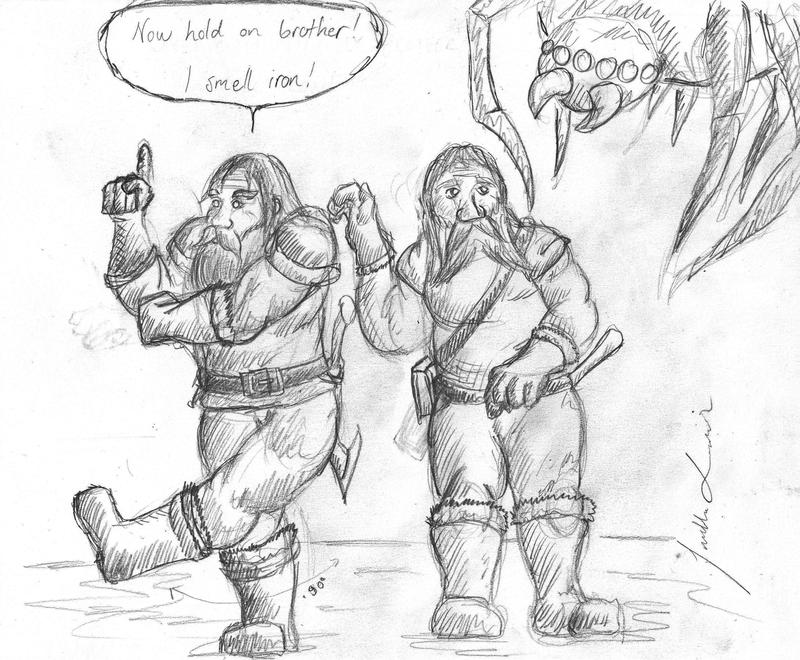
\includegraphics[width=.75\textwidth]{./resources/dandon}
  \caption{Dan and Don, two Gully dwarf brothers that rescued Cort from the
  mines.}
\end{figure}

The comedic duo of Dan and Don amused and exasperated Cort to no end during the
weeks he spent healing at their house. But nonetheless, Cort was touched by the
kindness of the two individuals, and after he got well, he brought the two of
them to the academy and hired them as his assistants, trying to ensure they had
a good life. They're probably his only two good friends from his life in
Thorbardin, he occasionally worries about their or their descendents fate to
this day.

\subsection{Grandmaster Urkhan}

\begin{figure}[!htb]
  \centering
  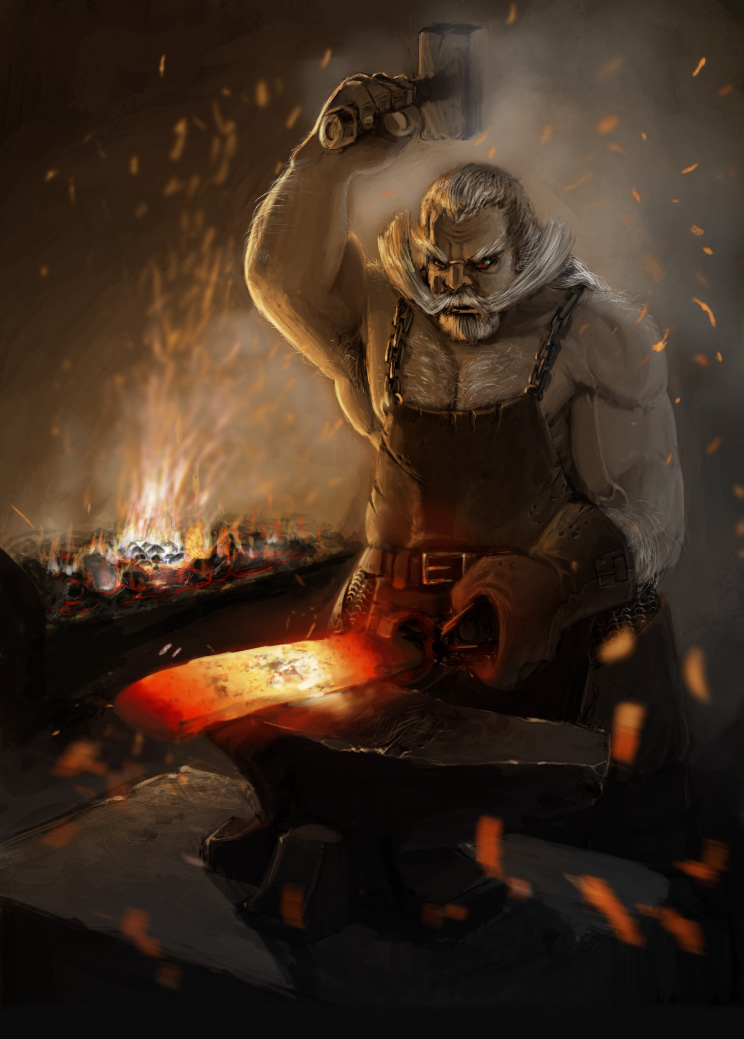
\includegraphics[width=.5\textwidth]{./resources/urkhan}
  \caption{Grandmaster Urkhan, Cort's master and father figure.}
\end{figure}

The good grandmaster took Cort in when he was young and taught him his current
skills in crafting. Although Cort never quite got to his level of artisanry, he
feeld deeply indebted to the man, for making him the man he was today.
Throughout his apprenticeship, Urkhan stressed how that the tools, the methods
and even the materials of the process of crafting all ultimately bowed to the
artist's vision, and the first thing that he must hone is his imagination. It's
because of these words that Cort was able to overcome his culturally drilled
hatred to magic, after seeing it's potential. With regards to the academy he
left behind, although the members there too abandoned him in the grandmaster
arena, he would still probably try to help them if he can.

\subsection{Tarkos Ireheart}

\begin{figure}[!htb]
  \centering
  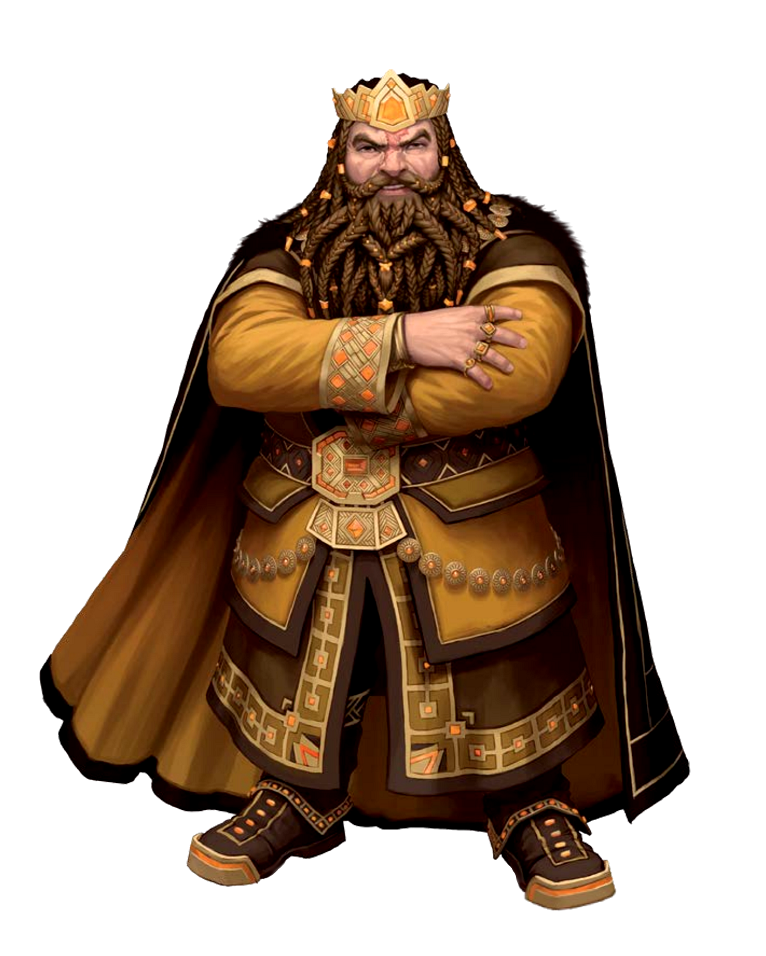
\includegraphics[width=.6\textwidth]{./resources/tarkos}
  \caption{Tarkos Ireheart, the hateful head of the Ireheart clan who banished
  Cort.}
\end{figure}

Tarkos was the clan head of the Ireheart clan of Thorbardin 200 years ago, and
then he was reponsible for exiling Cort after his display of magic in the
grandmaster proving arena. It's unknown whether this decision was his alone or
the clan's, but regardless, it's left Cort with a deep seated hatred for his
clan. Although he might be able to forgive the clan if they repent their
decision, he certainly will not forgive Tarkos for what he did to his hands, and
if Tarkos has already passed, then Cort's grudge will transfer to the next clan
head.

\end{document}
